\section{The motivation: feedback organization rules - uncovering the functions of feedback}
\label{subsec:subcsectionE}

 Understanding feedback mechanisms and organization is an important step in advancing the comprehension of the numerous functions it has been implicated with \cite{TopDown}: attention, awareness, working and associative memory, perceptual task, object expectation, prediction, scene segmentation, efference copy, perceptual learning.
Furthermore, their role in cortical computation remains to be explained, in particular within the frame of theories of hierarchical cortical computation.

In recent work \cite{Marques2018}, the aim was to bring about organization rules that can constrain and suggest theories of feedback function. 
The problem approached was the organizational logic of feedback axons relaying inputs from the lateromedial visual area (LM) to the lower area V1 in mice. LM is one of the main sources of feedback input into V1 and is also a retinotopically organized map of the visual field.

For this, RFs in LM-feedback boutons into V1 were mapped and related to those of neurons in their V1 vicinity.

Firstly, in layers L1 and L5/6 - layers to which feedback information is diffusely relayed to, in the target area V1, with diverse feedback signals \cite{9Marques2018kk} - LM visual area inputs targeted, on average, retinotopically matched locations in V1, meaning that the connections were, on the average effect, from neurons that map RFs close to those RFs that the target neurons represented. 

Despite this average organization, there was a high scattering of LM inputs in V1, with a large number of the considered LM feedback axons relaying visual information from distant points in the visual space. Thus, in a given location in V1, neurons have access to information from a wide area of the visual space from LM feedback inputs, with in fact a significant proportion of inputs coming from neurons coding deviations larger than $30º$ in the corresponding visual field.

Then the question turned to assessing if these deviations depended on the tuning properties of the LM boutons. The idea is that, in accounts to direction selective neurons, tuning-dependent wiring biases could relay predictive feedback signals of moving stimuli - image \ref{move}.

\begin{figure}[h]
\center
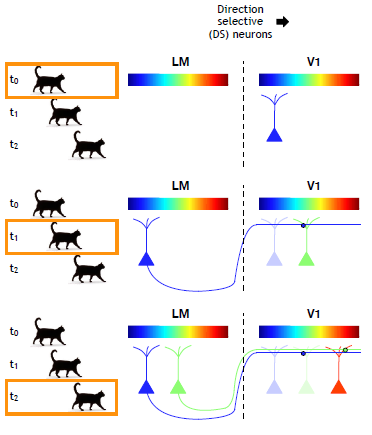
\includegraphics[scale=0.8]{2.Chapter/move.png}
\caption{Feedback signals from LM to V1 could convey predictive information about a moving object, if we consider that their wiring is biased according to their own tuning. In this example, we consider direction selectivity tuning as the criteria for the feedback wiring. \newline \textbf{Top:} A stimulus (the cat) moving in a given direction (left to right) will activate neurons in V1 with that direction selectivity and with their receptive fields located at the corresponding region where the stimulus is in the subject's visual field at that time $t_0$ (left-side, blue labeled azimuth angle). \newline \textbf{Middle:} These DS left field-of-view corresponding neurons feedforward to neurons whose RF represents the same left-side location in the visual field. These would project back into V1 neurons corresponding to positions on the middle region (green-labeled azimuth angle) activated by the stimulus at $t_1$. \newline \textbf{Down: } These neurons, activated by the stimuli presentation in that visual field region, also connect retinotopically to LM cells with the same direction selectivity. Again, these project to the neurons corresponding to the RF position ahead (right-side, red-labeled azimuth angle), activated by the stimulus at $t_2$). \newline In this way, predictions on the next cat's position, as assumed by the direction it followed at previous times, could be relayed via feedback from LM to V1 neurons.
\newline \newline \tiny{Image from the presentation by the principal co-author of \cite{Marques2018}, Tiago Marques, under the Champalimaud Internal Seminar Series on October $15^{th}$ 2017, \textit{The functional organization of cortical feedback}.}\label{cat}} 
\label{move}
\end{figure}

Different orientation selective neurons are intermingled in L1 of V1. This allows the simultaneous analysis and comparison of the effects of various tuning properties.

The experimental results showed that the retinotopic deviations depend on the feedback orientation and direction selectivities, according to simple geometrical rules - figure \ref{rules}.

Orientation-selective (OS) LM axons overspread around the retinotopically matched location in V1, and target neurons that encode positions perpendicular to the LM neurons' preferred orientation. Additionally, analysis on direction-selective (DS) axons presented that these overspread to areas with neurons encoding positions shifted from the retinotopically matched position along the angle of the LM neurons' anti-preferred direction. 

In this way, LM feedback axons could enhance visual representations in space and time, by targeting cells in V1 that code positions placed perpendicularly to the higher-level neuron's orientation selectivity or to positions placed in the opposite direction to the higher-level neuron's direction selectivity. These differ from the predictive coding hypothesis (image \ref{move}), that relied on neurons that feedback to lower-area neurons encoding positions that would be subsequent according to the stimuli direction. Instead, the work of \cite{Marques2018},  showed that feedback neurons do have organizational structure that relates to their tuning properties, but that the feedback targeting is to neurons encoding the \textit{opposite} position to that expected to be visually stimulated at following moments by the moving stimuli that drove the input neurons in the first place, when in a new position. 

\begin{figure}[H]
\center
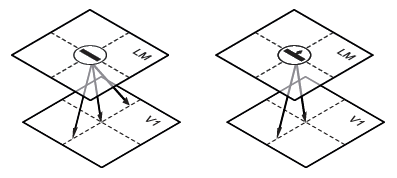
\includegraphics[scale=0.8]{2.Chapter/rules.PNG}
\caption{LM feedback to V1 functional organization according to simple geometrical rules. Planes represent retinotopic maps in V1 and LM, while bars represent preferred orientation of the LM neurons. \newline \textbf{Left:} OS inputs have biased wiring towards neurons encoding positions orthogonal to the input feedback neurons preferred orientation.
\newline \textbf{Right:} DS inputs tend to be wired to neurons that encode visual field positions along the opposite direction to the feedback input neuron's preferred motion direction.
\newline \newline \tiny{Images from \cite{Marques2018}.}}
\label{rules}
\end{figure}

This could also manifest a predictive coding strategy, but in the negative, with feedback wiring to cells that care about the non-expected positions. This could for example be explained if the wiring portraits a net inhibitory effect.

In broader terms, this study showed that there are asymmetries in the way that feedback connections are established, and that these asymmetries depend on the tuning properties of the involved cells. 
Given the possible relation of feedback and SM effects, this motivated the scope of this project: to unravel the anisotropies and asymmetries of SM effects with moving stimuli and put them at the perspective of the possible connection circuits that could cause them.
